%%%%%%%%%%%%%%%%%%%%%%%%%%%%%%%%%%%%%%%%%
% baposter Landscape Poster
% LaTeX Template
% Version 1.0 (11/06/13)
%
% baposter Class Created by:
% Brian Amberg (baposter@brian-amberg.de)
%
% This template has been downloaded from:
% http://www.LaTeXTemplates.com
%
% License:
% CC BY-NC-SA 3.0 (http://creativecommons.org/licenses/by-nc-sa/3.0/)
%
%%%%%%%%%%%%%%%%%%%%%%%%%%%%%%%%%%%%%%%%%

%----------------------------------------------------------------------------------------
%	PACKAGES AND OTHER DOCUMENT CONFIGURATIONS
%----------------------------------------------------------------------------------------

\documentclass[landscape,a0paper,fontscale=0.285]{baposter} % Adjust the font scale/size here

\usepackage{graphicx}
\usepackage{sidecap}


\usepackage{floatrow}
\graphicspath{{figures/}} % Directory in which figures are stored

\usepackage{amsmath} % For typesetting math
\usepackage{amssymb} % Adds new symbols to be used in math mode

\usepackage{booktabs} % Top and bottom rules for tables
\usepackage{enumitem} % Used to reduce itemize/enumerate spacing
\usepackage{palatino} % Use the Palatino font
\usepackage[font=small,labelfont=bf]{caption} % Required for specifying captions to tables and figures

\usepackage{multicol} % Required for multiple columns
\setlength{\columnsep}{1.5em} % Slightly increase the space between columns
\setlength{\columnseprule}{0mm} % No horizontal rule between columns

\usepackage{tikz} % Required for flow chart
\usetikzlibrary{shapes,arrows} % Tikz libraries required for the flow chart in the template

\newcommand{\compresslist}{ % Define a command to reduce spacing within itemize/enumerate environments, this is used right after \begin{itemize} or \begin{enumerate}
\setlength{\itemsep}{1pt}
\setlength{\parskip}{0pt}
\setlength{\parsep}{0pt}
}

\definecolor{columbiablue}{rgb}{0.61, 0.87, 1.0}
\definecolor{lightblue}{rgb}{0.145,0.6666,1} % Defines the color used for content box headers
\definecolor{darkblue}{rgb}{0.0, 0.0, 0.55}

\begin{document}

\begin{poster}
{
headerborder=closed, % Adds a border around the header of content boxes
colspacing=1.5em, % Column spacing
bgColorOne=columbiablue!40, % Background color for the gradient on the left side of the poster
bgColorTwo=columbiablue!40, % Background color for the gradient on the right side of the poster
borderColor=darkblue, % Border color
headerColorOne=darkblue, % Background color for the header in the content boxes (left side)
headerColorTwo=darkblue, % Background color for the header in the content boxes (right side)
headerFontColor=white, % Text color for the header text in the content boxes
boxColorOne=white, % Background color of the content boxes
textborder=roundedsmall, % Format of the border around content boxes, can be: none, bars, coils, triangles, rectangle, rounded, roundedsmall, roundedright or faded
eyecatcher=true, % Set to false for ignoring the left logo in the title and move the title left
headerheight=0.1\textheight, % Height of the header
headershape=smallrounded, % Specify the rounded corner in the content box headers, can be: rectangle, smallrounded, roundedright, roundedleft or rounded
headerfont=\Large\bf\textsc, % Large, bold and sans serif font in the headers of content boxes
%textfont={\setlength{\parindent}{1.5em}}, % Uncomment for paragraph indentation
linewidth=2pt % Width of the border lines around content boxes
}
%----------------------------------------------------------------------------------------
%	TITLE SECTION 
%----------------------------------------------------------------------------------------
%
{
\includegraphics[height=5em]{nsf.png}} % First university/lab logo on the left
{\bf\textsc{Improving Bayesian methods for locating breakpoints in time series}\vspace{0.5em}} %poster title
% \\ \smallskip
{\textsc{ {\LARGE Madison Ell$^{1}$, Dainia Higgins$^{2}$, Sarah Klingbeil$^{3}$, Nathaniel Wilson$^{2}$ \hspace{12pt} }  } }%\\ \smallskip {\large  This research is funded by National Science Foundation grant number \#1560222.}}  % Author names and institution
{
\includegraphics[height=3em]{lafayette-college.png}} % Second university/lab logo on the right

%----------------------------------------------------------------------------------------
%	INTRODUCTION
%----------------------------------------------------------------------------------------

\headerbox{Introduction}{name=introduction,column=0,row=0, span=2}{

Our project presents new approaches to finding the quantity and location of breakpoints in time series data. These methods take in account for structural changes which allows for more appropriate data modeling. Bayesian Adaptive Auto-Regression (BAAR) is a Bayesian technique that samples from a distribution of the number and location of breakpoints. New sets of breakpoints are proposed by a reversible-jump Markov Chain Monte Carlo process and are then evaluated using a Metropolis-Hasting algorithm. Simulation results show that BAAR detected the number and location of breakpoints with accuracy that met and sometimes exceeded the performance of the existing frequentist methods.
 %Jeff question

\vspace{0.3em} % When there are two boxes, some whitespace may need to be added if the one on the right has more content
}


%----------------------------------------------------------------------------------------
%	METHODS
%----------------------------------------------------------------------------------------

\headerbox{Methods}{name=method,column=0,below=introduction, span =2}{ % This block's bottom aligns with the bottom of the conclusion block
\begin{multicols}{2}
\textbf{Initial Breakpoint(s):} BAAR uses results from Bai-Perron$^{[1]}$ constrained to a maximum of 2 breakpoints combined with a burn-in period of at least 2 times the number of data points.
\\

\textbf{Step Type:}
Inspired by the BARS$^{[3]}$ technique, our Markov Chain Monte Carlo has 3 different step types: Birth, Death, and Move which encompasses 2 options called Jump and Jiggle. 
\begin{itemize}\compresslist
\item Birth: Random addition of a breakpoint. 
\item Death: Random deletion of a breakpoint.
\item Move: Either Jump or Jiggle.
\end{itemize}

\textit{Jump:} A randomly chosen existing breakpoint is moved to a random new location. \\

\begin{center}
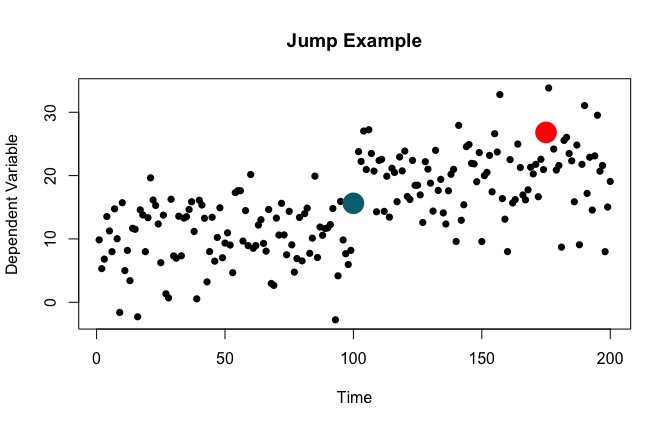
\includegraphics[width=.55\linewidth]{jump_example}
\captionof{figure}{An example of Jump on simulated data. Existing breakpoint is in teal, and proposed is in red.}
\end{center}

\textit{Jiggle:} A randomly chosen existing breakpoint is moved to a location within a restricted interval around the original location. It is calculated by $J_n = (x_b-\rho n, x_b+\rho n)$, where $n$ is the length of data and $\rho$ is the percent of data in the interval. 
\begin{center}
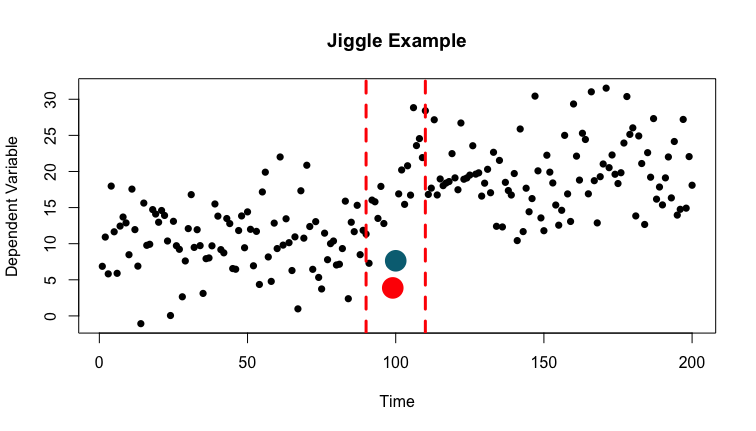
\includegraphics[width=.55\linewidth]{jiggle_example}
\captionof{figure}{ An example of Jiggle on simulated data with $\rho = 0.05$ and $J_n = (90,110)$. Existing breakpoint at $t = 100$ is in teal, and proposed at $t = 99$ is in red.}
\end{center}


%\end{multicols}

%----------------------------------------

%\begin{multicols}{2}

\textbf{The Metropolis-Hastings Ratio:} Determines the acceptance of proposed breakpoints. BIC is used to approximate the Bayes factor$^{[2]}$, which streamlines the equation: 
\begin{equation}
log(r) \approx \Big( \frac{- \Delta BIC}{2}\Big) \frac{\pi (\tau_n,K_n)}{\pi(\tau_o,K_o)} \frac{q(\tau_o K_o | \tau_nK_n)}{q(\tau_n K_n | \tau_oK_o)}
\end{equation}
where $r$ is the acceptance probability, $K$ and $\tau$ are the number and location of breakpoints, $q$ is the proposal density, and $\pi$ is the prior information. 

\end{multicols}
}


%----------------------------------------------------------------------------------------
%	RESULTS
%----------------------------------------------------------------------------------------

\headerbox{Results}{name=results,column=2,span=2,row=0}{

\begin{multicols}{2}
\vspace{0.5em}

\begin{center}
\includegraphics[width=.73\linewidth]{plot2.png}
\captionof{figure}{{\small Simulated data used to test BAAR method with one significant break at $t = 45$. For $t \leq 45$, $y_t = -0.7 y_{t-1} +\epsilon_t$ and for $t > 45$ $y_t = 0.7 y_{t-1} +\epsilon_t$}. }
\end{center}

\begin{center}
\includegraphics[width=.73\linewidth]{Breakpoints Number Mean_Standard Devation=1,Breakpoint at 45.png}
\captionof{figure}{{\small Average number of breakpoints obtained from a $1,000$ iteration run from varying AR-1 coefficients} }
\end{center}

\end{multicols}
%------------------------------------------------
\begin{multicols}{2}
\vspace{0.5em}

In the simulated data set (Figure 3), BAAR accurately finds the location of the single breakpoint (Figure 4). Due to the clarity of the breakpoint in the training data, BAAR places a high probability of it existing at exactly time point 100 while still accepting some other possibilities.

\end{multicols}

}


%----------------------------------------------------------------------------------------
%	case study
%----------------------------------------------------------------------------------------

\headerbox{Case Study: Suicide Among People Ages 15-24 in the U.S.A.}{name=caseStudy, column=2, span=2, row=0, below=results, bottomaligned=method}{

\begin{multicols}{2}
\vspace{1em}
Suicide is the fourth leading cause of death among Americans ages 15 to 24$^{[4]}$. BAAR accurately models the suicide counts among people ages 15 to 24 in the United States of America as 4 subsections (Figure 5), locating breakpoints between 1995 and 1996, 2002 and 2003, and 2007 through 2013 that correspond to the economic prosperity of the 1990s, the dot-com economic crash, and the Great Recession (Figure 6).

\end{multicols}

%------------------------------------------------

\begin{multicols}{2}
\vspace{1em}
\begin{center}
\captionof{figure}{Suicide counts among American people ages 15 to 24: navy blue circles - true values; orange squares - fitted values from single AR(2).}
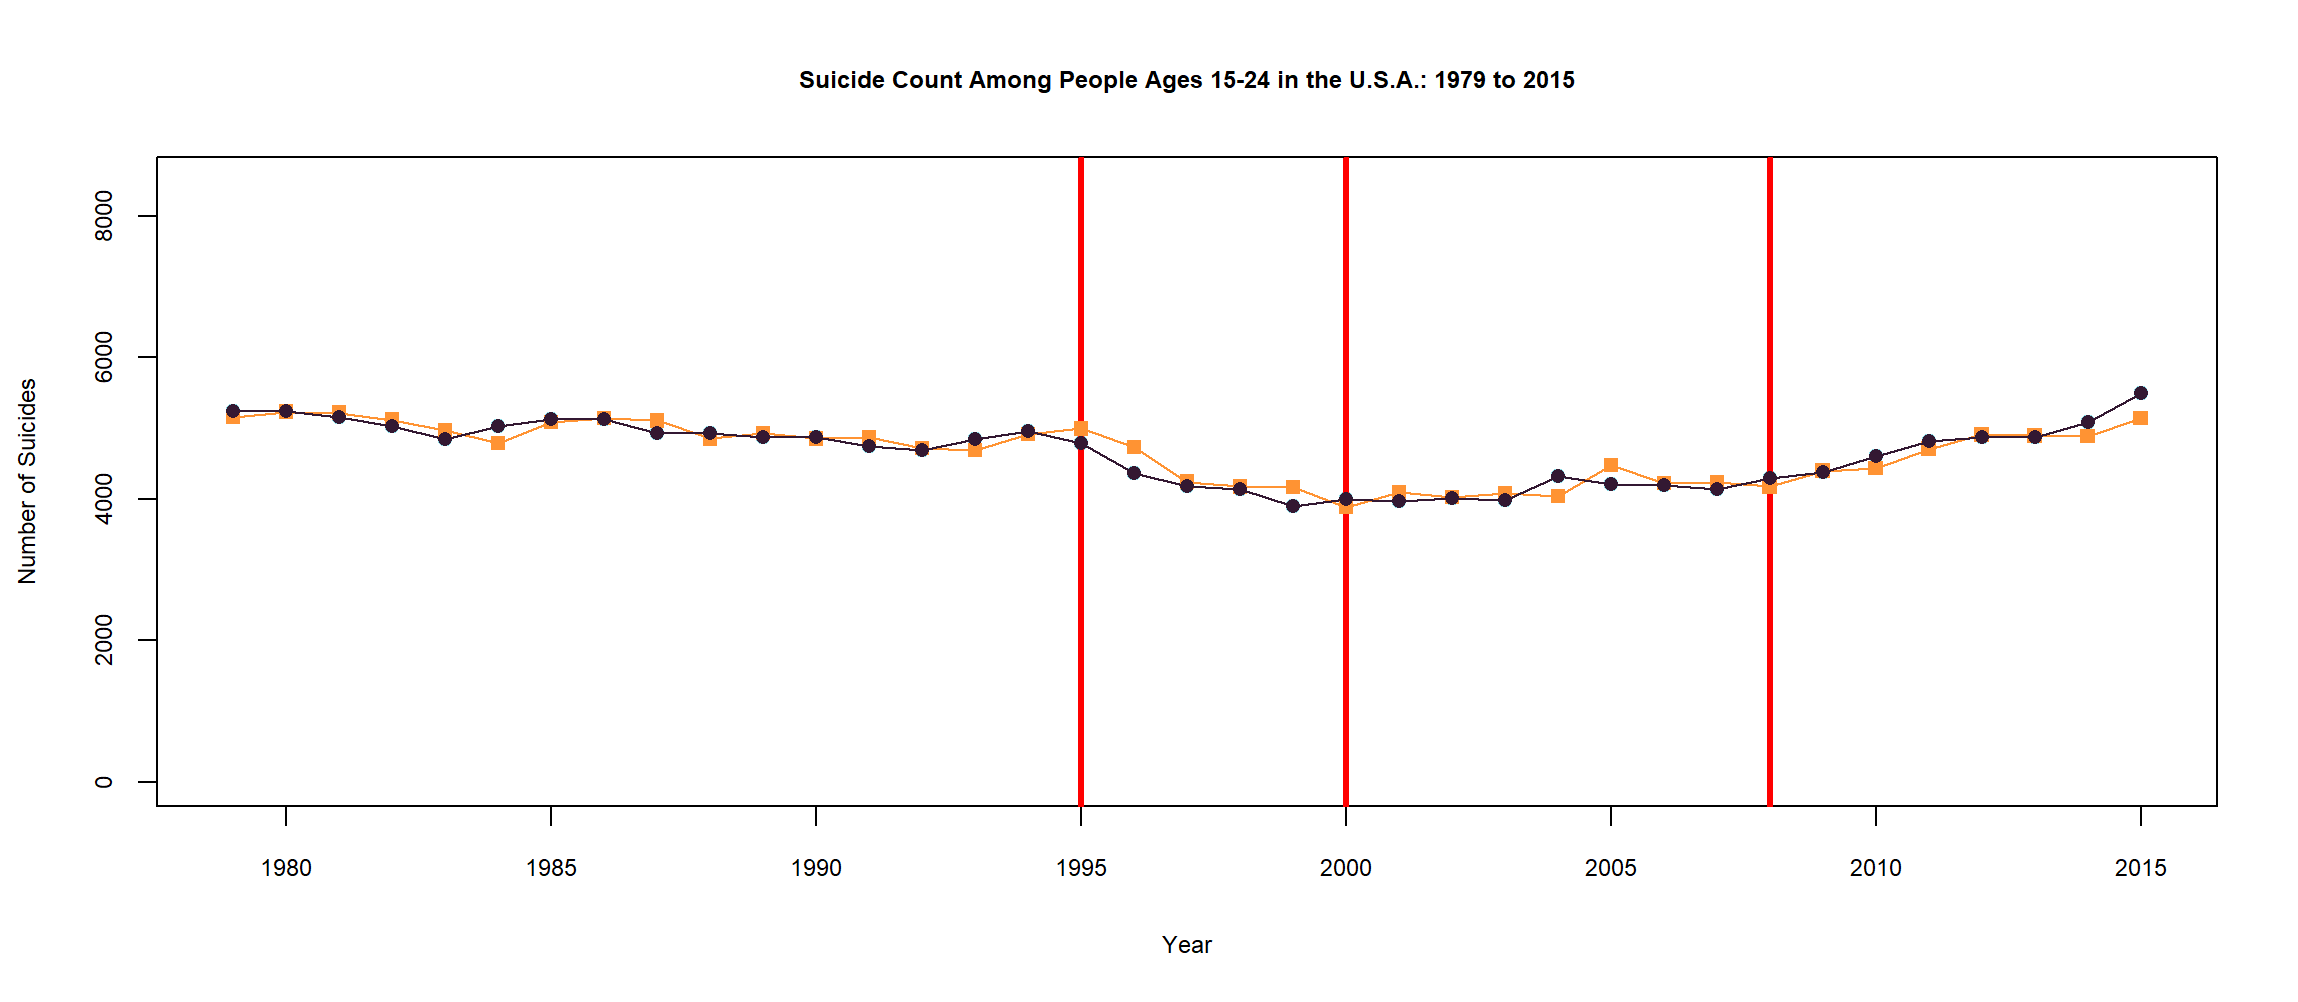
\includegraphics[width=.75\linewidth]{suiciddee.jpg}
\captionof{figure}{Distribution of breakpoint locations in suicide data among 15-24 year olds in the United States of America.}
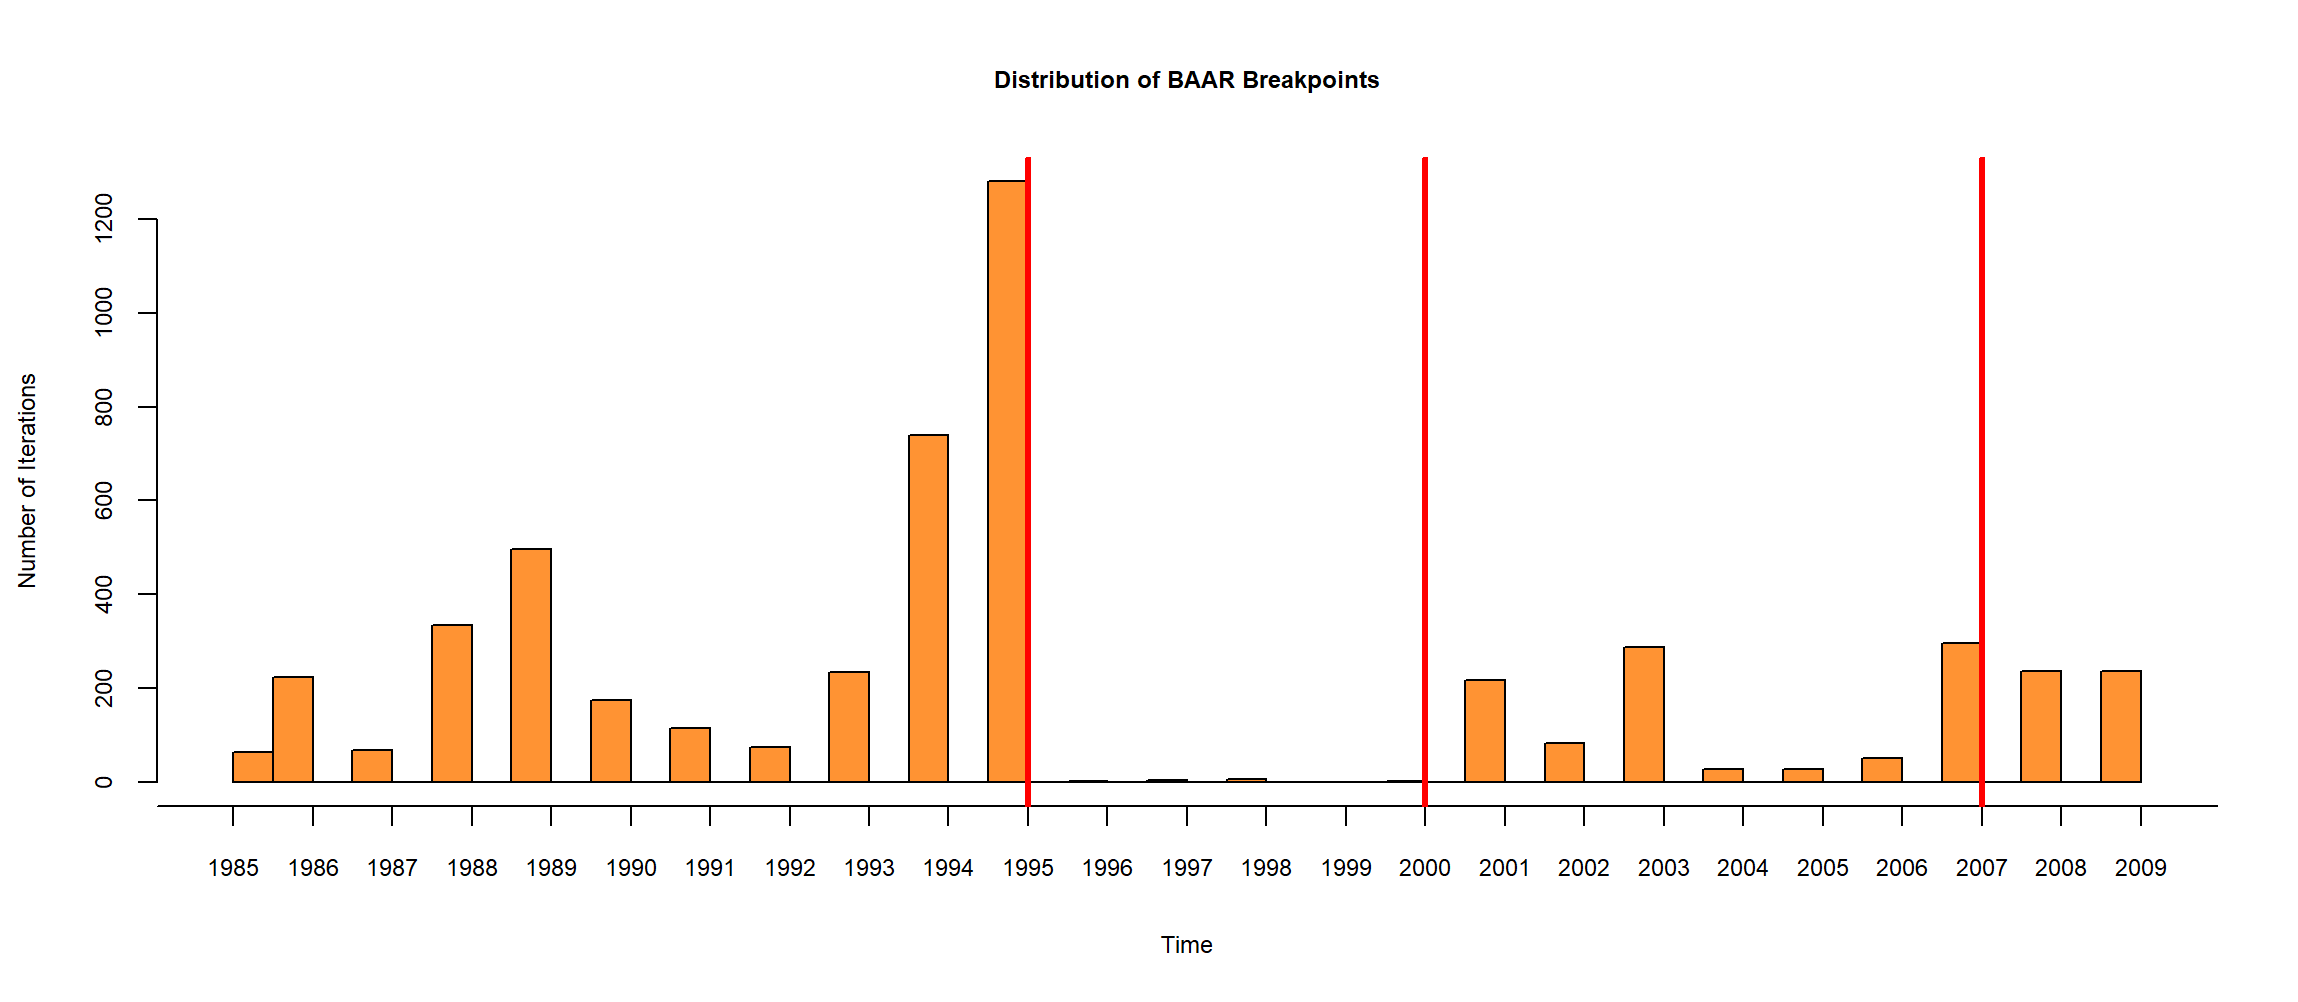
\includegraphics[width=0.9\linewidth]{suiciddee2.jpg}
\end{center}

\end{multicols}
}


%----------------------------------------------------------------------------------------
%	REFERENCES
%----------------------------------------------------------------------------------------

\headerbox{References}{name=references,column=1,span=2,above=bottom}{ % This block is as tall as the references block
\begin{multicols}{2}
\renewcommand{\section}[2]{\vskip 0.05em} % Get rid of the default "References" section title
\nocite{*} % Insert publications even if they are not cited in the poster

%\small{ % Reduce the font size in this block 
\footnotesize{
\begin{description}
\item[${[1]}$] Bai, J. and Perron, P., (2003). \textit{Computation and analysis of multiple structural change models}. Journal of applied econometrics, 18(1), pp.1-22. 
\item[${[2]}$] Kass, R.E. and Wasserman, L., (1995). \textit{A reference Bayesian test for nested hypotheses and its relationship to the Schwarz criterion}. Journal of the american statistical association, 90(431), pp.928-934. 
\item[${[3]}$] DiMatteo, I., Genovese, C.R. and Kass, R.E., (2001). \textit{Bayesian curve-fitting with free-knot splines}. Biometrika, 88(4), pp.1055-1071.
\item[${[4]}$] World Health Organization, (2016).\textit{Self-inflicted injuries}. WHO Mortality Database.

\end{description}
}
%scriptsize :smaller text
\end{multicols}
}

%----------------------------------------------------------------------------------------
%	AFFILIATIONS
%----------------------------------------------------------------------------------------

\headerbox{Affiliations}{name=affiliations,column=3,aligned=references,above=bottom}{ % This block is as tall as the references block

\begin{description}\compresslist
\scriptsize {\item{ Department of Mathematics, Lafayette College}}
\scriptsize{\item { This research is funded by the National Science Foundation, grant number \#2150343}}
 \scriptsize {\item[$^1$]{ Mathematics and Computer Science Division,  Fullerton College }}
\scriptsize {\item[$^2$]{Department of Mathematics and Computer Science, Coppin State University}}
\scriptsize { \item[$^3$]{ Mathematics Department/English Department, Southern Adventist University}}
\end{description}
}

%----------------------------------------------------------------------------------------
%	CONTACT INFORMATION
%----------------------------------------------------------------------------------------

\headerbox{Contact Information}{name=contact,column=0,aligned=references,above=bottom}{ % This block is as tall as the references block
\begin{description}\compresslist
\item[\textbf{Emails:}] 
\item madison.ell4@gmail.com
\item DHiggins00@student.coppin.edu
\item klingbeil.sarah@gmail.com 
\item NWilson10@student.coppin.edu
\end{description}
}



%----------------------------------------------------------------------------------------
%	RESULTS 
%----------------------------------------------------------------------------------------

%\headerbox{Results}{name=results,column=0,span = 2, below=method,bottomaligned=caseStudy}{ % This block's bottom aligns with the bottom of the conclusion block


%}

%----------------------------------------------------------------------------------------

\end{poster}

\end{document}
